\documentclass[10pt,a4paper]{article}
\usepackage[T1]{fontenc}
\usepackage[utf8]{inputenc}
\usepackage{lmodern,microtype}
\usepackage[a4paper,margin=1.85cm]{geometry}
\usepackage{amsmath,amssymb,xcolor,enumitem,setspace,graphicx}
\usepackage[hidelinks]{hyperref}
\usepackage{tikz}
\usetikzlibrary{positioning,arrows.meta,calc}
\definecolor{titleblue}{HTML}{005293}
\setlength{\parindent}{1.25em}
\setlength{\parskip}{0pt}
\setlength{\emergencystretch}{2em}
\setstretch{1.04}
\setlist{itemsep=1pt,topsep=3pt,leftmargin=1.6em}
\pagestyle{empty}

\begin{document}
\begin{center}
{\Large\bfseries\color{titleblue}Physics-Guided Graph Learning for Conductive-Particle Allocation\par
in Polydisperse Packed Beds\par}
\vspace{0.7em}
{\normalsize Research concept proposal\par}
\vspace{0.25em}
{\small Ali Khalifa and Heiko Briesen\par
Technical University of Munich, Chair of Process Systems Engineering\par}
\end{center}
\vspace{0.45em}

\begin{abstract}
Heat transfer through particle beds is important in many natural and industrial systems, including the heating, cooling, drying and temperature control of granular materials, as well as thermal-energy storage. Adding a small amount of highly
conductive material may help, but its location can be as important as its
amount. This study asks where conductive particles should be placed when the
packing geometry, porosity, particle-size distribution and conductive-material
volume must remain fixed. DEM will generate mechanically valid packings. A
steady thermal-network solver will test candidate material allocations, while
a repeated swap search will create strong reference solutions. A graph neural
network (GNN) will then learn which particles are useful within the contact
network. For a new packing, it will rank the particles that should receive the
limited high-conductivity material. One final thermal solve will verify the
proposed allocation. The study will test whether this fast graph-based rule can
outperform random placement and simple physics-based rankings while avoiding
most of the repeated search.
\end{abstract}

\section{Motivation and research question}
Heat travels through a packed bed along connected particle contacts. Conductive
particles are therefore useful only when their locations support heat transport
between the hot and cold boundaries. Random mixing may waste material in weakly
used regions. Choosing only particles with many contacts may also fail because
such particles can lie on side branches that carry little heat.

The central question is therefore:
\begin{quote}\itshape
With the packing and amount of conductive material fixed, where should the
conductive particles be placed, and can a GNN make this decision for a new bed?
\end{quote}
Figure~\ref{fig:problem} shows the task. DEM fixes the particle positions, sizes
and contacts. We change only which particles are labelled as high conductivity.
The study therefore measures the effect of placement alone.

\begin{figure}[!ht]
\centering
\resizebox{0.64\textwidth}{!}{%
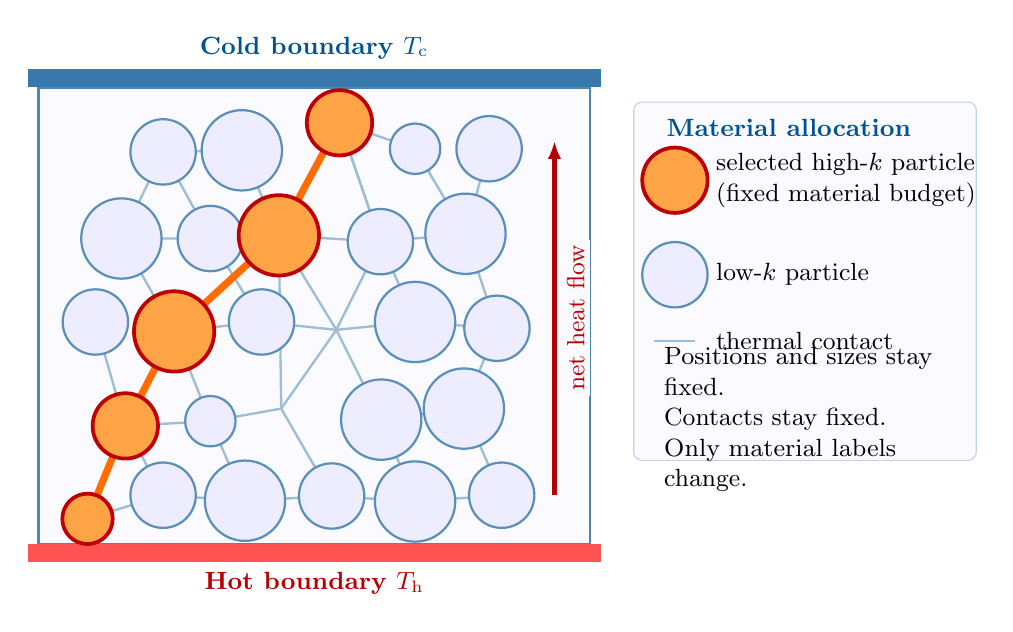
\begin{tikzpicture}[
 lowS/.style={circle,draw=titleblue!65,fill=blue!7,line width=0.8pt,minimum size=6.4mm,inner sep=0pt},
 lowM/.style={circle,draw=titleblue!65,fill=blue!7,line width=0.8pt,minimum size=8.3mm,inner sep=0pt},
 lowL/.style={circle,draw=titleblue!65,fill=blue!7,line width=0.8pt,minimum size=10.2mm,inner sep=0pt},
 highS/.style={circle,draw=red!75!black,fill=orange!72,line width=1.35pt,minimum size=6.4mm,inner sep=0pt},
 highM/.style={circle,draw=red!75!black,fill=orange!72,line width=1.35pt,minimum size=8.3mm,inner sep=0pt},
 highL/.style={circle,draw=red!75!black,fill=orange!72,line width=1.35pt,minimum size=10.2mm,inner sep=0pt},
 contact/.style={draw=titleblue!38,line width=0.85pt},
 path/.style={draw=orange!85!red,line width=2.6pt,line cap=round},
 heat/.style={-{Latex[length=2.3mm]},red!72!black,line width=1.6pt},
 label/.style={align=left,font=\small}]

% Domain and thermal boundaries
\fill[blue!2] (0,0) rectangle (7,5.8);
\draw[titleblue!70,line width=1pt] (0,0) rectangle (7,5.8);
\fill[red!68] (-0.14,-0.23) rectangle (7.14,0);
\fill[titleblue!78] (-0.14,5.8) rectangle (7.14,6.03);
\node[font=\small\bfseries,text=red!72!black] at (3.5,-0.50) {Hot boundary $T_{\mathrm h}$};
\node[font=\small\bfseries,text=titleblue] at (3.5,6.30) {Cold boundary $T_{\mathrm c}$};

% Contact network, drawn behind the particles
\draw[contact] (0.62,0.32)--(1.10,1.50)--(1.72,2.70)--(3.05,3.92)--(3.82,5.35);
\draw[contact] (0.62,0.32)--(1.58,0.62)--(1.10,1.50)--(2.18,1.56)--(1.72,2.70);
\draw[contact] (1.58,0.62)--(2.62,0.55)--(2.18,1.56)--(3.08,1.72)--(3.05,3.92);
\draw[contact] (2.62,0.55)--(3.72,0.61)--(3.08,1.72)--(3.78,2.72)--(3.05,3.92);
\draw[contact] (3.72,0.61)--(4.78,0.54)--(4.35,1.58)--(3.78,2.72);
\draw[contact] (4.78,0.54)--(5.88,0.62)--(5.40,1.72)--(4.35,1.58);
\draw[contact] (0.72,2.82)--(1.10,1.50)--(1.72,2.70)--(1.05,3.88)--(1.58,4.98);
\draw[contact] (1.72,2.70)--(2.83,2.82)--(2.18,3.88)--(3.05,3.92);
\draw[contact] (2.83,2.82)--(3.78,2.72)--(4.34,3.84)--(3.82,5.35);
\draw[contact] (3.78,2.72)--(4.78,2.82)--(4.34,3.84)--(5.42,3.94);
\draw[contact] (4.78,2.82)--(5.82,2.74)--(5.40,1.72)--(4.35,1.58);
\draw[contact] (5.82,2.74)--(5.42,3.94)--(5.72,5.02);
\draw[contact] (1.05,3.88)--(2.18,3.88)--(1.58,4.98)--(2.58,5.00)--(3.05,3.92);
\draw[contact] (3.05,3.92)--(4.34,3.84)--(3.82,5.35)--(4.78,5.02)--(5.42,3.94);

% Highlight one candidate conductive route behind the selected particles
\draw[path] (0.62,0.32)--(1.10,1.50)--(1.72,2.70)--(3.05,3.92)--(3.82,5.35);

% Low-conductivity particles: three clearly visible size classes
\node[lowM] at (1.58,0.62) {}; \node[lowL] at (2.62,0.55) {};
\node[lowM] at (3.72,0.61) {}; \node[lowL] at (4.78,0.54) {};
\node[lowM] at (5.88,0.62) {}; \node[lowS] at (2.18,1.56) {};
\node[lowL] at (4.35,1.58) {}; \node[lowL] at (5.40,1.72) {};
\node[lowM] at (0.72,2.82) {}; \node[lowM] at (2.83,2.82) {};
\node[lowL] at (4.78,2.82) {}; \node[lowM] at (5.82,2.74) {};
\node[lowL] at (1.05,3.88) {}; \node[lowM] at (2.18,3.88) {};
\node[lowM] at (4.34,3.84) {}; \node[lowL] at (5.42,3.94) {};
\node[lowM] at (1.58,4.98) {}; \node[lowL] at (2.58,5.00) {};
\node[lowS] at (4.78,5.02) {}; \node[lowM] at (5.72,5.02) {};

% Selected particles forming the illustrated pathway
\node[highS] at (0.62,0.32) {}; \node[highM] at (1.10,1.50) {};
\node[highL] at (1.72,2.70) {}; \node[highL] at (3.05,3.92) {};
\node[highM] at (3.82,5.35) {};

% Net heat-flow direction
\draw[heat] (6.55,0.62)--(6.55,5.12);
\node[font=\small,rotate=90,text=red!72!black,fill=blue!2,inner sep=2pt]
 at (6.82,2.87) {net heat flow};

% Compact legend panel
\node[draw=titleblue!25,fill=blue!2,rounded corners=3pt,
 minimum width=4.35cm,minimum height=4.55cm,anchor=north west] at (7.55,5.62) {};
\node[font=\small\bfseries,text=titleblue,anchor=west] at (7.85,5.28) {Material allocation};
\node[highM] at (8.08,4.62) {};
\node[label,anchor=west] at (8.48,4.62) {selected high-$k$ particle\\(fixed material budget)};
\node[lowM] at (8.08,3.42) {};
\node[label,anchor=west] at (8.48,3.42) {low-$k$ particle};
\draw[contact] (7.82,2.58)--(8.34,2.58);
\node[label,anchor=west] at (8.48,2.58) {thermal contact};
\node[label,anchor=west,text width=3.6cm,font=\small] at (7.82,1.58)
{Positions and sizes stay fixed.\\Contacts stay fixed.\\Only material labels change.};
\end{tikzpicture}%
}
\caption{Inverse allocation problem in a polydisperse packed bed. The orange
particles illustrate one possible conductive path; finding useful allocations
is the subject of the proposed study, not an assumed result.}
\label{fig:problem}
\end{figure}

\newpage
\section{Hypothesis and objectives}
The working hypothesis is:
\begin{quote}\setstretch{1.10}\itshape
Good allocations depend on connected paths through several particles. A GNN
should recognize these paths better than rules that score each particle only
from its own properties or number of contacts.
\end{quote}
This is a hypothesis to be tested, not an assumed result. The objectives are to:
\begin{enumerate}
\item measure how much particle placement matters at a fixed material budget;
\item create strong reference allocations using repeated thermal calculations;
\item test whether a GNN can propose good allocations for unseen beds; and
\item identify the contact-network structures that form useful heat paths.
\end{enumerate}

\section{\hspace{0.25em}Proposed hybrid modelling framework}
Each component has one clear role:
\begin{center}
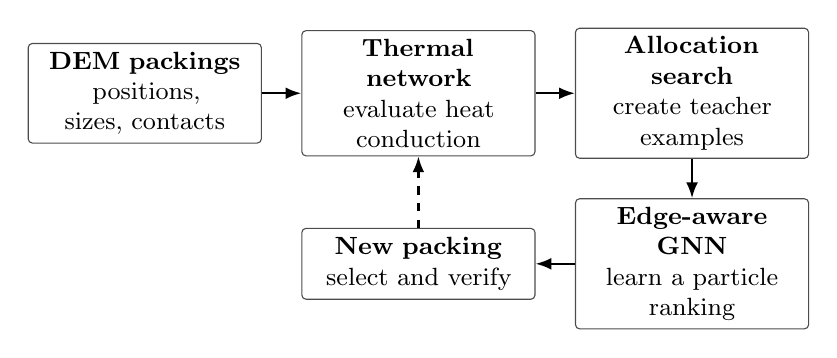
\begin{tikzpicture}[node distance=5mm,
 box/.style={draw=black!70,rounded corners=1.5pt,minimum height=9mm,text width=2.75cm,align=center,font=\small,inner sep=3pt},
 arr/.style={-{Latex[length=2mm]},thick}]
\node[box] (dem) {\textbf{DEM packings}\\positions, sizes, contacts};
\node[box,right=of dem] (thermal) {\textbf{Thermal network}\\evaluate heat conduction};
\node[box,right=of thermal] (search) {\textbf{Allocation search}\\create teacher examples};
\node[box,below=of search] (gnn) {\textbf{Edge-aware GNN}\\learn a particle\\ranking};
\node[box,left=of gnn] (new) {\textbf{New packing}\\select and verify};
\draw[arr] (dem)--(thermal); \draw[arr] (thermal)--(search);
\draw[arr] (search)--(gnn); \draw[arr] (gnn)--(new); \draw[arr,dashed] (new)--(thermal);
\end{tikzpicture}
\end{center}

\paragraph{WP1: Controlled packing ensemble.}
Generate independent polydisperse DEM beds with the same number of particles,
size distribution and target porosity. The allowed number and size classes of
high-conductivity particles remain the same in every case.

\paragraph{WP2: Thermal solver and physics-guided search.}
Solve steady heat conduction on the contact network and calculate the effective
conductivity. Repeatedly exchange one selected and one unselected particle of
the same size class. This fixed-budget swap search produces strong training
examples while keeping particle count, size distribution and material volume
unchanged.

\paragraph{WP3: Graph-learning model.}
Represent particles as graph nodes and their thermal contacts as edges. For a
new packing, the GNN assigns one usefulness score to every particle. Particles
are ranked separately within each size class, and the highest-ranked particles
receive the available high-conductivity material. Thus, the GNN predicts
\emph{where to place the material}; it does not generate the packing itself.

\paragraph{WP4: Transfer test and mechanism analysis.}
Keep complete packings unseen during training. On each unseen bed, compare the
GNN allocation with random placement, contact-number ranking, a simple
heat-path ranking and the swap search. Verify every proposed allocation with
the same thermal solver and inspect the resulting heat paths.

\section{\hspace{0.25em}Expected contribution, scope and decision criterion}
The expected contribution is a fast material-allocation method for disordered
particle beds. The thermal solver determines which allocations work, the swap
search creates reference examples, and the GNN makes this knowledge reusable
for new beds. Unlike a model that only predicts effective conductivity, the GNN
selects concrete particles, so its proposed paths can be inspected directly.

The first study will isolate stationary solid-contact conduction. Convection,
radiation, particle motion and application-specific material constraints will
remain outside the initial scope. They can be added if the controlled study
shows that allocation is important.

The GNN is useful only if, on unseen packings, it consistently performs better
than random placement and the simple rankings, recovers a meaningful part of
the swap-search improvement, and needs far fewer thermal solves. If a simple
rule performs equally well, the study will show that the GNN is unnecessary.
\end{document}
